% File name: Manual.tex

\documentclass[]{jsarticle}

\usepackage{graphicx} %画像用のパッケージ
\usepackage{color} %文字カラー用のパッケージ
\usepackage{url} %URL用のパッケージ
\usepackage{ascmac} %枠などのパッケージ


\title{WebAlbumGenerator マニュアル}
\author{kengo92i}
\date{2014年08月08日}

\begin{document}
\maketitle

% 目次の表示
%\tableofcontents

% 表目次の表示
%\listoftables

% 図目次の表示
%\listoffigures




\section{はじめに}

\subsection{概要}
「 WebAlbumGenerator 」はWebアルバムページを自動生成してくれるソフトウェアです。貴方はもうWebアルバムを作るのに時間をかける必要はありません。写真をフォルダにまとめて、タイトルと日付を書いたら、クリック1つでWebアルバムページが完成します。旅行やイベントの思い出などを貴方もWebページとして公開してみませんか?必要なのは"思い出"だけ。HTMLやCSS、そしてJavaScriptの知識は必要ありません。それは「 WebAlbumGenerator 」の仕事です。

\subsection{ライセンスについて}
「 WebAlbumGenerator 」はThe MIT Licenseによって保護されています。\\

\begin{itembox}[l]{The MIT License}
 \begin{itemize}
   \item このソフトウェアを誰でも無償で無制限に扱って良い。ただし、著作権表示および本許諾表示をソフトウェアのすべての複製または重要な部分に記載しなければならない。
   \item 作者または著作権者は、ソフトウェアに関してなんら責任を負わない。
 \end{itemize}
\end{itembox} \\

上記の内容に基づいて、本ソフトウェアは保護されています。基本的には自由に扱う事が出来ますが、上記のライセンスを違反するような行為は禁止されています。原文や詳細な内容はソフトウェアに付属している「 LICENSE.txt 」をご覧ください。

\subsection{動作環境}
「 WebAlbumGenerator 」はMacOSX用のアプリとして開発されています。WindowsやLinuxなどのOSはサポートしていません。
推奨環境としては以下のようになっています。\\

\begin{itembox}[l]{推奨環境}
 \begin{itemize}
   \item MacOSX : 10.9.4
   \item Python : 2.7.5
 \end{itemize}
\end{itembox} \\

上記を満たしていない場合の動作は確認していませんが、多分大丈夫だと思います。また、WindowsやLinuxへの対応は未定となっています。

\section{使い方}

\subsection{ソフトウェアのインストール}

公式サイトより、「 WebAlbumGenerator.dmg 」をダウンロードし、起動します。すると、図\ref{fig:ex1}のような画面が表示されます。
表示されたウィンドウ内で、「 WebAlbumGenerator.app 」のアイコンをドラッグし、「 Applications 」のエイリアスの上で離します。\\

\begin{figure}[htbp] %図の挿入
 \begin{center}
  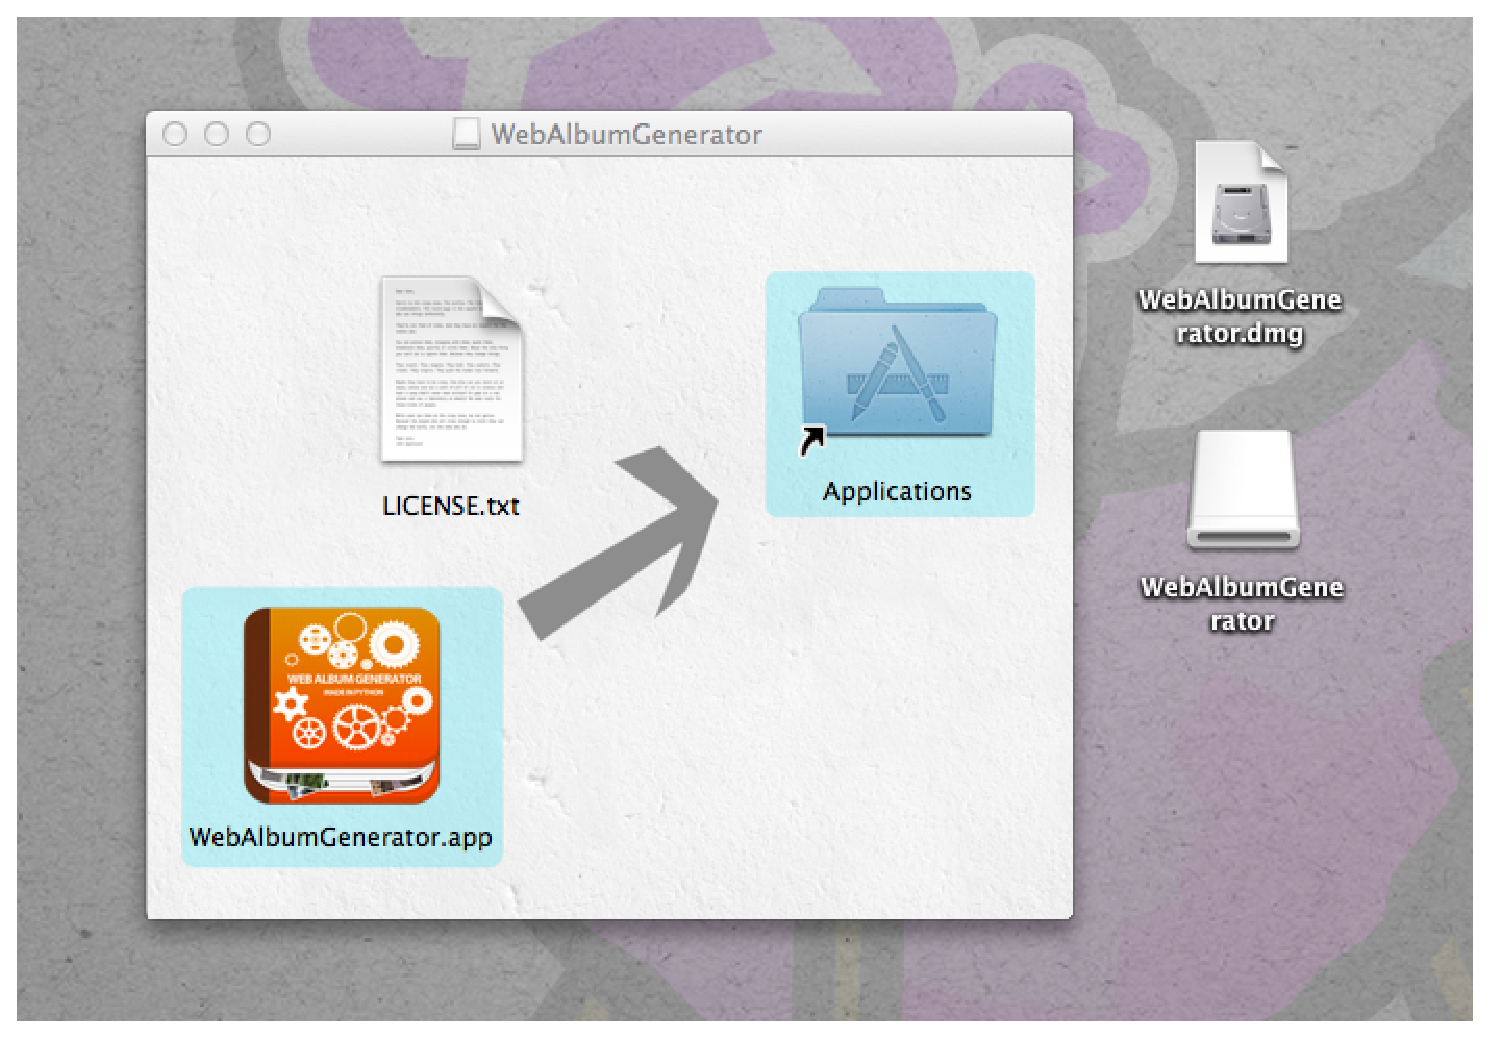
\includegraphics[width=120mm]{images/ex1.eps}
 \end{center}
 \caption{ソフトウェアのインストール}
 \label{fig:ex1}
\end{figure}

この作業を行う事で、PC内の「 Applications 」フォルダに「 WebAlbumGenerator.app 」が保存されます。以降は普通のアプリケーションと
同じく実行できるようになります。\newpage

\subsection{使用する画像を選ぶ}

ソフトウェアのインストールが終了した後、アルバムページに使用する画像を1つのフォルダにまとめます(図\ref{fig:ex2})。
図\ref{fig:ex2}では、デスクトップに「 images 」というフォルダ作成し、使用する画像をまとめています。

\begin{figure}[htbp] %図の挿入
 \begin{center}
  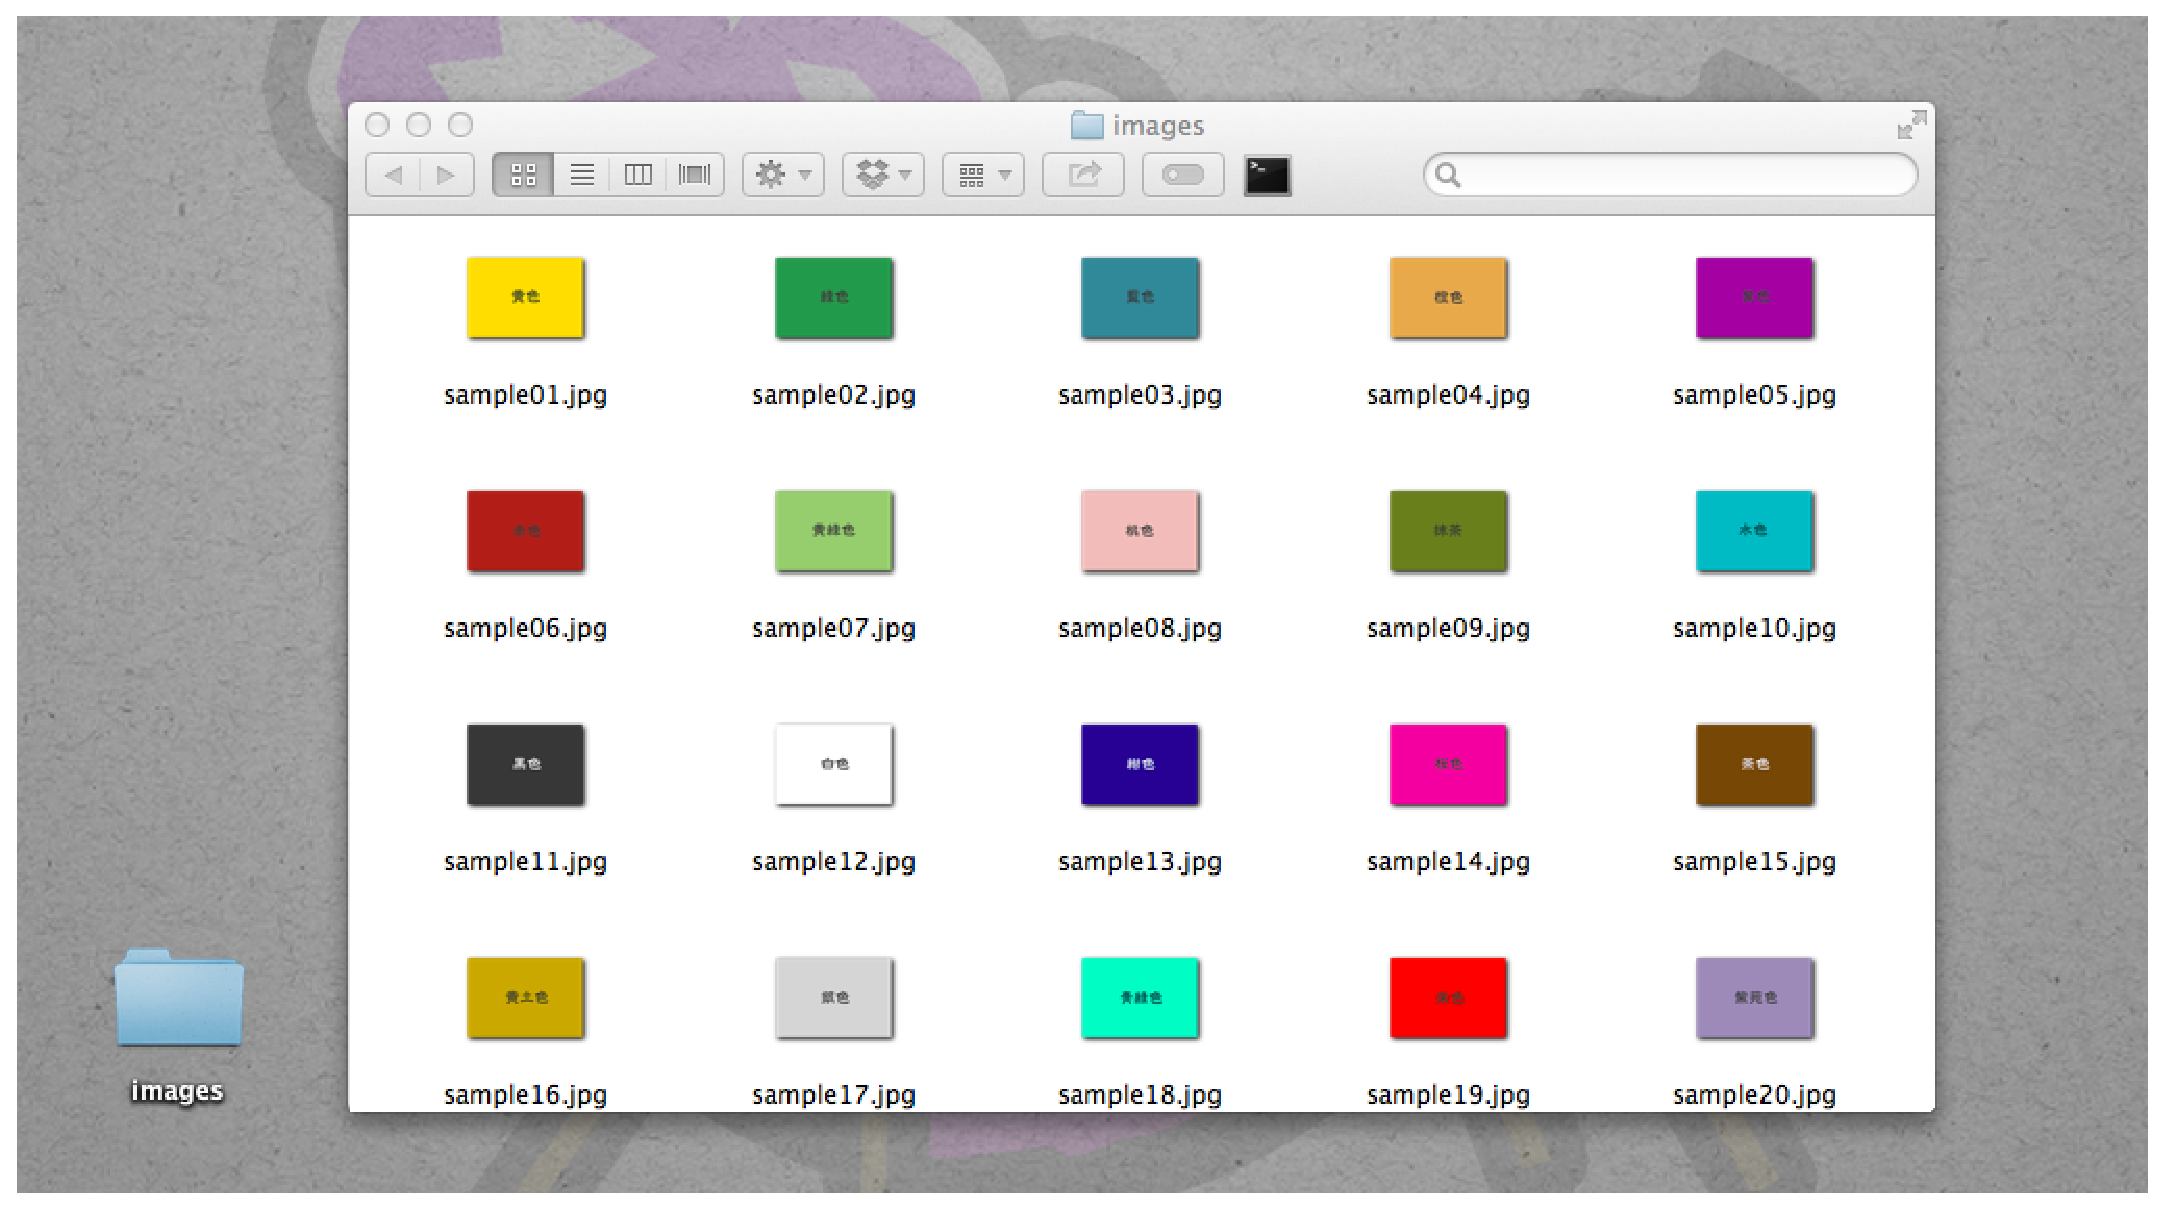
\includegraphics[width=120mm]{images/ex2.eps}
 \end{center}
 \caption{使用する画像をフォルダにまとめる}
 \label{fig:ex2}
\end{figure}

使用する画像の準備が整いました。ここから、Webアルバムを作成していきます。\\

\subsection{アプリケーションを実行する}

「 WebAlbumGenerator.app 」を実行すると、図\ref{fig:ex3}のようなウィンドウが表示されます。入力フォームに必要事項を入力し、
問題がなければ、ウィンドウ右下の「作成」をクリックします。\\

その後、さらにウィンドウが開かれ、フォルダ選択を求められます(図\ref{fig:ex4})。\\
図\ref{fig:ex4}の画面で、必要な画像をまとめたフォルダを選択します。選択したフォルダが問題なければ、「Choose」をクリックします。\\

フォルダ選択後、表示されているターミナル上に実行結果が表示されます。問題がなければ、デスクトップにWebアルバムが出力されます。

\begin{figure}[htbp] %図の挿入
 \begin{center}
  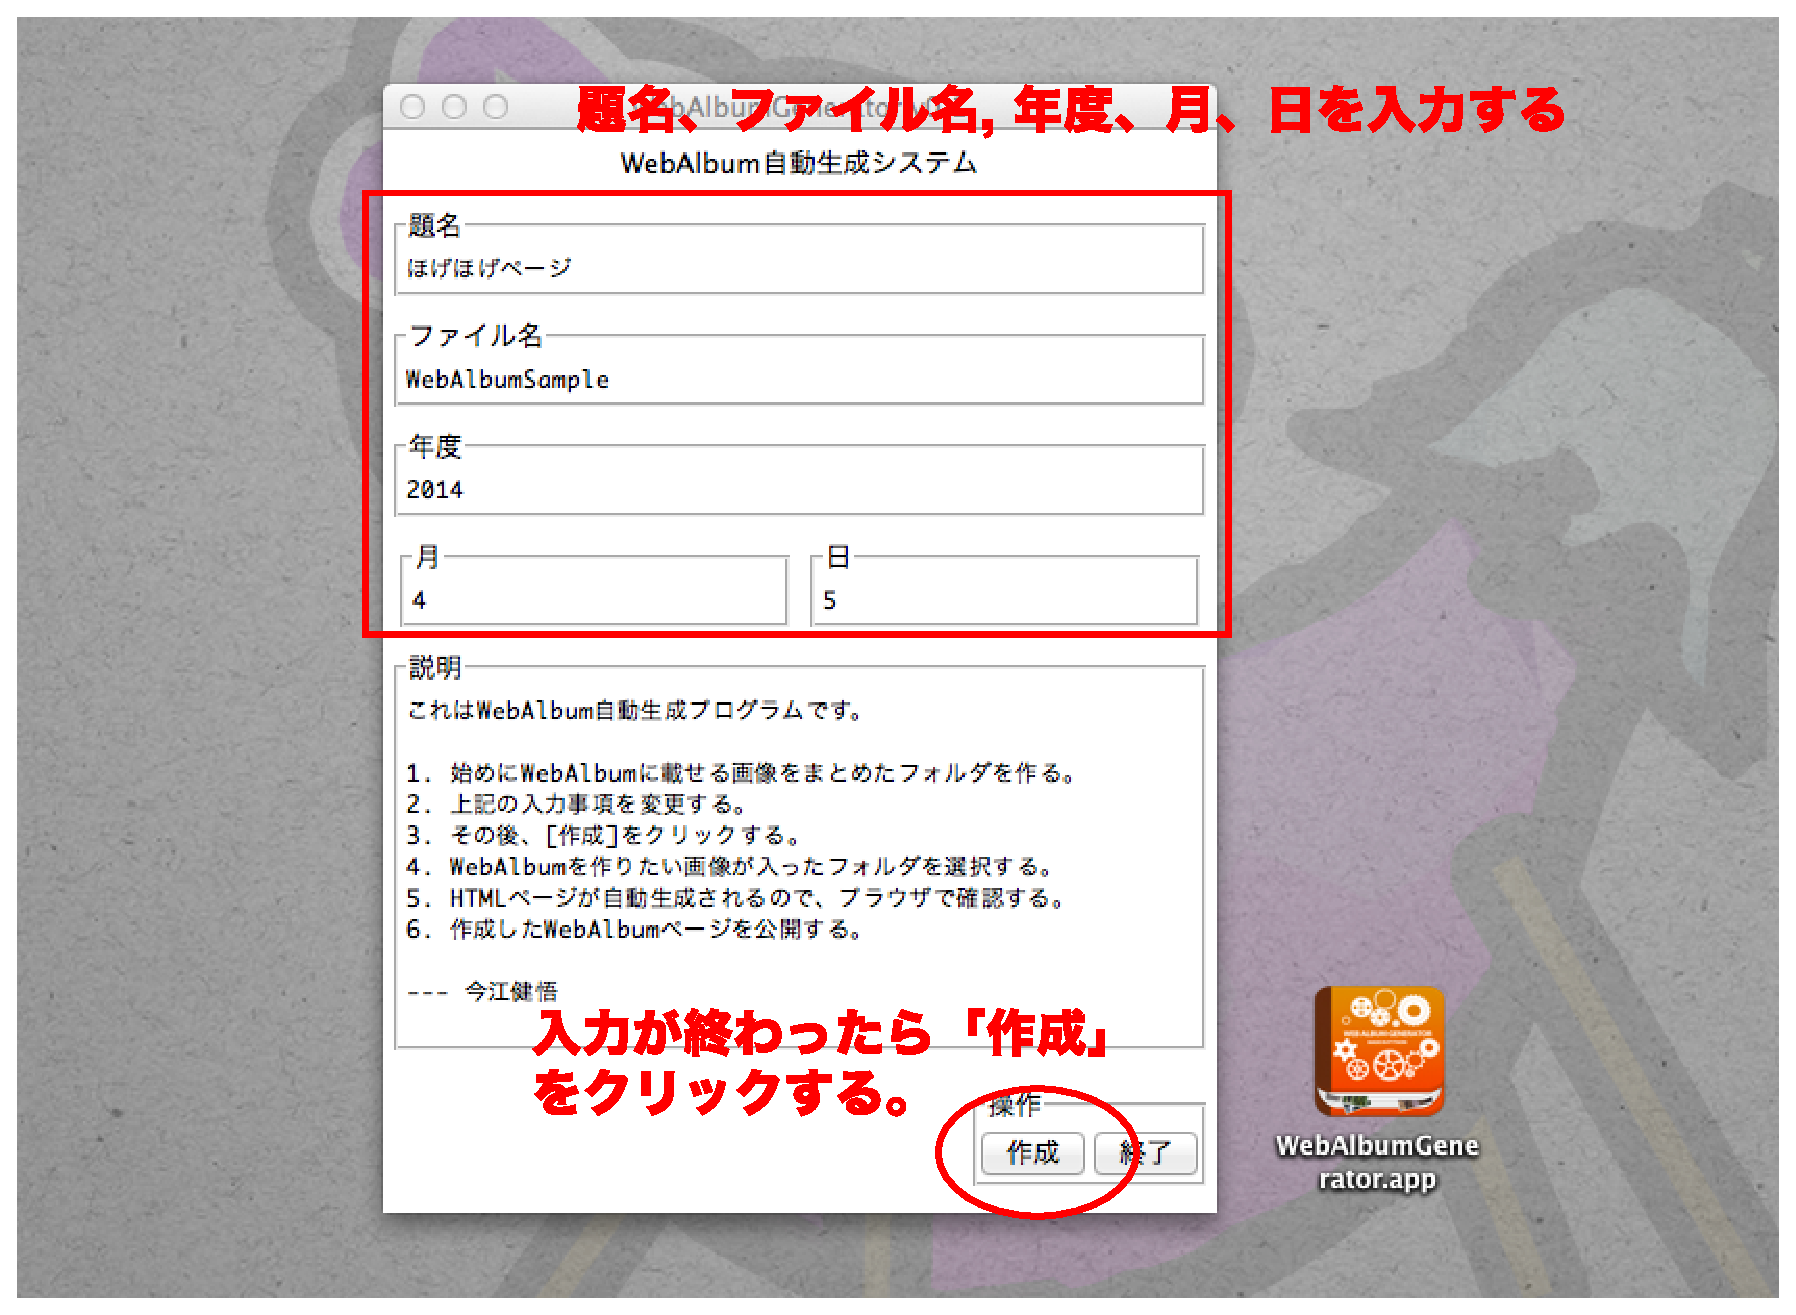
\includegraphics[width=120mm]{images/ex3.eps}
 \end{center}
 \caption{アプリケーション起動時に表示されるウィンドウ}
 \label{fig:ex3}
\end{figure}

\begin{figure}[htbp] %図の挿入
 \begin{center}
  \includegraphics[width=120mm]{images/ex4.eps}
 \end{center}
 \caption{フォルダ選択画面}
 \label{fig:ex4}
\end{figure}

\newpage

\subsection{出力されたWebアルバムについて}

実行時に問題がなければ、デスクトップに「WebAlbum」というフォルダが作成されています。もし、実行中に問題があった場合は、後述の
「不具合について」をご覧下さい。図\ref{fig:ex5}が「WebAlbum」フォルダの中身になります。

\begin{figure}[htbp] %図の挿入
 \begin{center}
  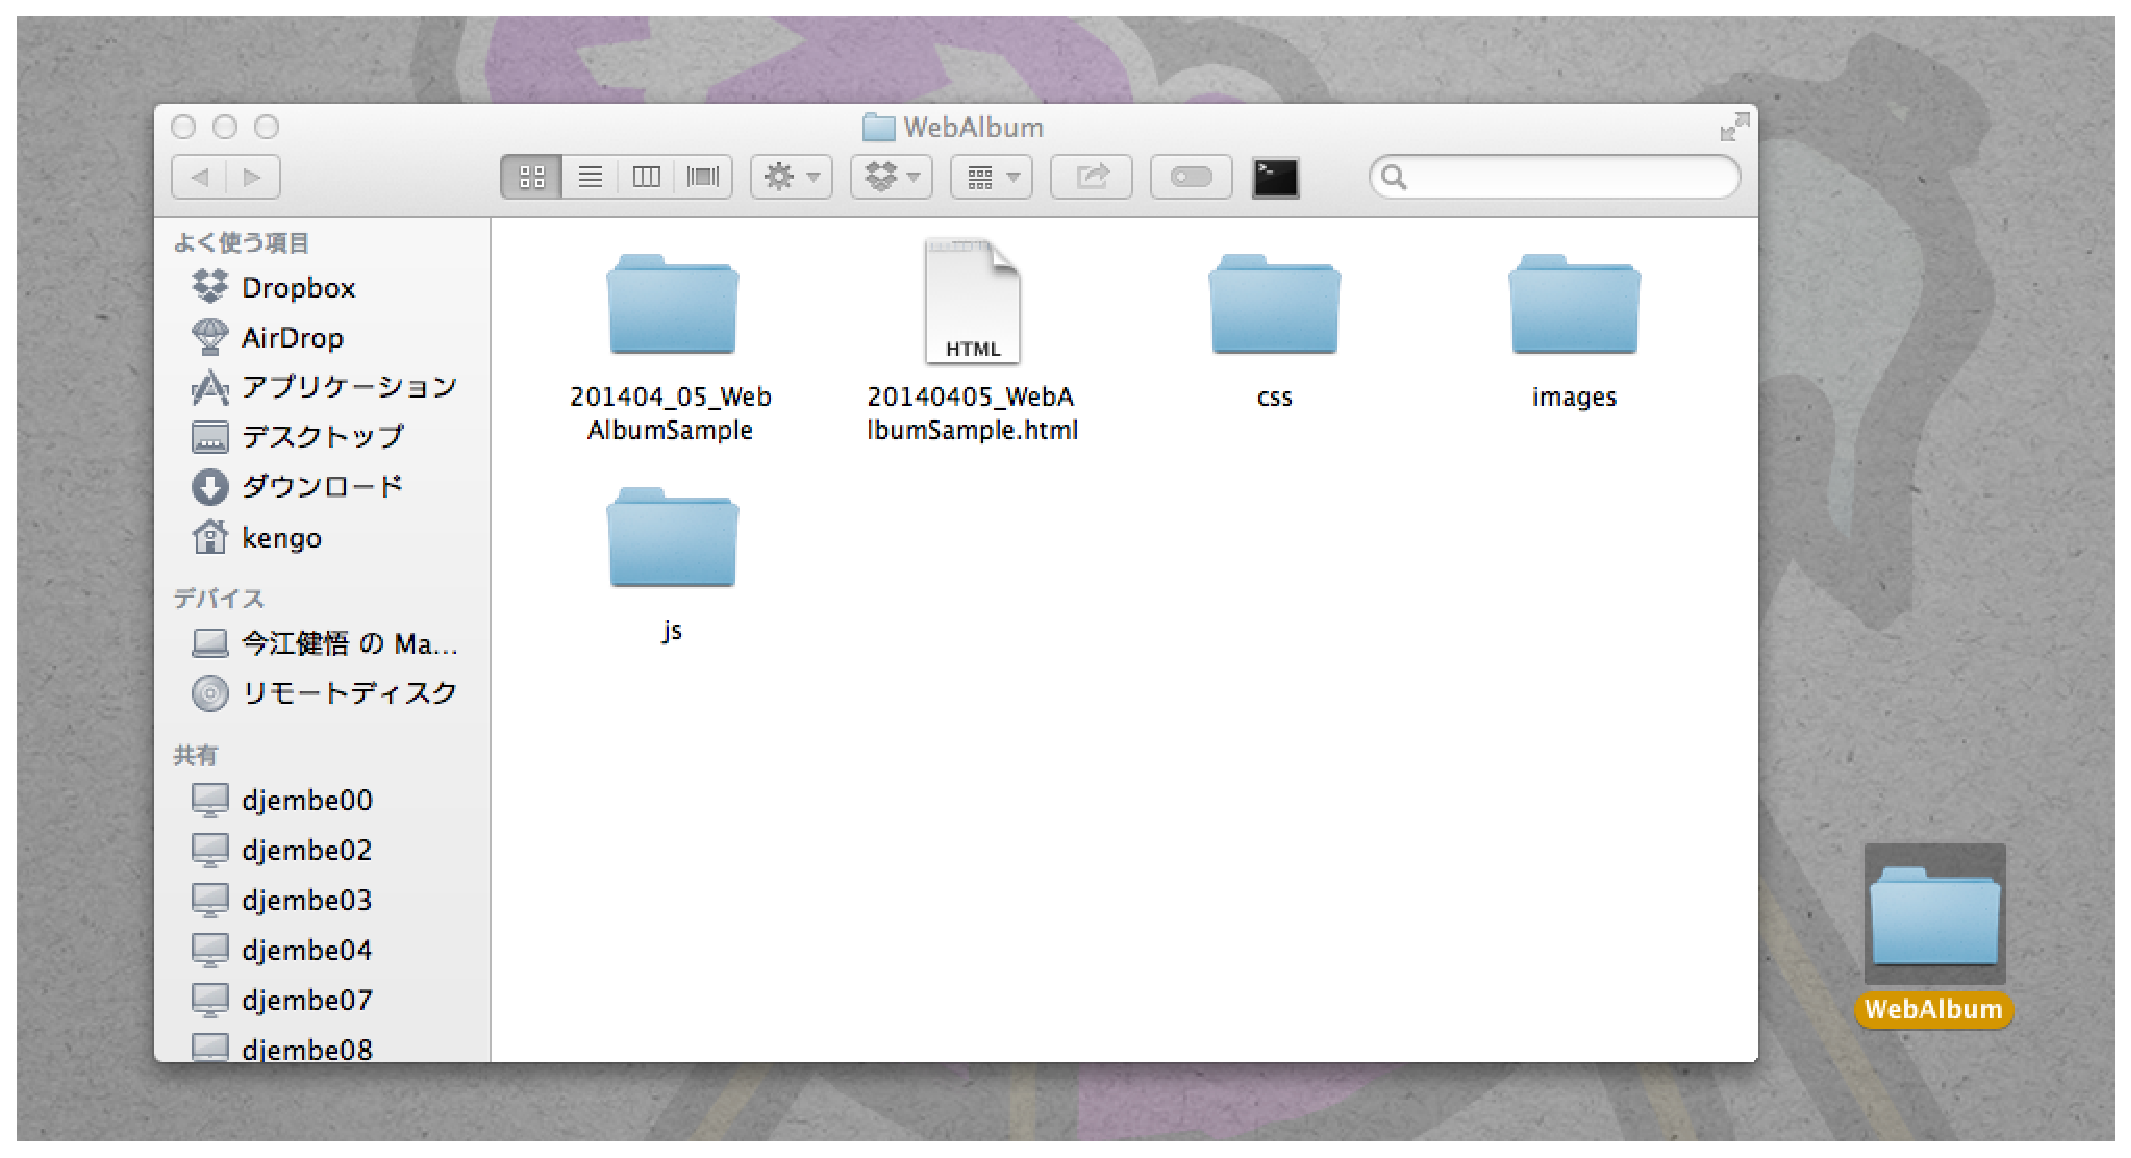
\includegraphics[width=120mm]{images/ex5.eps}
 \end{center}
 \caption{出力されたWebアルバムについて}
 \label{fig:ex5}
\end{figure}

\begin{itembox}[l]{「WebAlbum」フォルダの中身について}
 \begin{itemize}
   \item 201404\_05\_WebAlbumSample : Webアルバムページ用の画像とサムネイルが入っています。
   \item 20140405\_WebAlbumSample.html : WebアルバムページのHTMLファイルです。 
   \item css : 必要なcssファイル一式が入っています。
   \item images : Webアルバムページ用の画像が入ってます。
   \item js : Webアルバムページに必要なJavascriptファイルが入ってます。
 \end{itemize}
\end{itembox} 

※初期値で出力した場合のファイル名になっています。入力値を変えた場合はファイル名も変わります。\\

同じディレクトリ階層に複数のWebアルバムページを公開する場合は、「css」, 「images」,「js」はコピーする必要が
ありません。違うWebアルバムページでも上記のフォルダに関しては中身は同じものになっています。\\

上記の例で言うと、
「201404\_05\_WebAlbumSample」と「20140405\_WebAlbumSample.html」は出力するWebアルバムページによって
中身は違っているため、コピーする必要があります。

\newpage

\section{不具合について}

「WebAlbumGenerator」には不具合が存在しています。もし意図した通りに動作しない場合は以下の不具合に該当している可能性があります。
それぞれについて解説しているので、おかしな動作をした場合はご覧下さい。

\subsection{ディレクトリ指定のパス名に日本語ファイル名が含まれている場合の不具合}
必要な画像をまとめたフォルダが日本語ファイル名である場合や、ファイルを指定しているパスに日本語が含まれている場合が該当します。\\

\begin{itembox}[l]{日本語を含むパスの例について}
 \begin{itemize}
   \item /Users/Tanaka/Desktop/沖縄旅行の思い出
   \item /Users/Tanaka/Pictures/イベント/images 
 \end{itemize}
\end{itembox} 

\subsection{入力フォームへの日本語入力の不具合}

この問題に関して、入力フォームに日本語をうてないという不具合です。原因に関しては、PythonのGUIライブラリの仕様とのことです。
解決策としては、日本語文章をメモ帳などでうったものをコピペすると入力出来ます。Pythonの仕様です。すいません。解決策があれば
教えてもらえると助かります。\\

\subsection{その他日本語に関する不具合}
そのほかにも、日本語が使われていると動作しない可能性が高いです。まとめる画像ファイルに日本語名が入っている場合なども
動作しない原因になります。日本語の問題に関しては、Pythonの仕様によるところもあるため、Pythonの仕様ライブラリが日本語に
対応するのを待つ事になりそうです。\\

--- kengo92i

\end{document}


